\documentclass[11pt]{article}

\input{vsv_template_hdr.tex}

% Test of timecode functionality of the preview script.

\begin{doucment}

\begin{frame}{1-0:00}{1-5:00}{right}
\vsvhl{1-0:10}{1-0:20}{This frame is designed to test the ungreying of an environment, and then a bulleted list.}

\begin{vsvgrey}{1-0:30}{}
\lipsum[66]
\end{vsvgrey}

\begin{itemize}
\vsvitem{1-0:40}{}{grey}
\lipsum[74]
\vsvitem{1-0:50}{}{grey}
\lipsum[75]
\vsvitem{1-1:00}{}{grey}
\lipsum[74]
\vsvitem{1-1:10}{}{grey}
\lipsum[75]
\vsvitem{1-1:20}{}{grey}
\lipsum[74]
\vsvitem{1-1:50}{}{grey}
\lipsum[75]
\end{itemize}

\begin{vsvgrey}{1-2:00}{}
And then finally this environment will ungrey until the end of the frame.
\end{vsvgrey}

\end{frame}

\begin{frame}{1-0:00}{1-5:00.10}{left}
\vsvhl{1-0:9.50}{1-00:020.60}{This frame is designed to test code correction.}

TODO: put some code here

% TODO: put a description list here
\end{frame}


\begin{frame}{1-5:00}{1-10:00.01}{right}
\vsvhl{1-5:10}{1-5:20}{This frame is designed to test appearance of items in a list and image includes.}

\begin{vsvappear}{1-5:30}{}
This text will appear! Hello cruel world, from this paragraph!
\end{vsvappear}

\begin{enumerate}
\vsvitem{1-5:40}{}{appear}
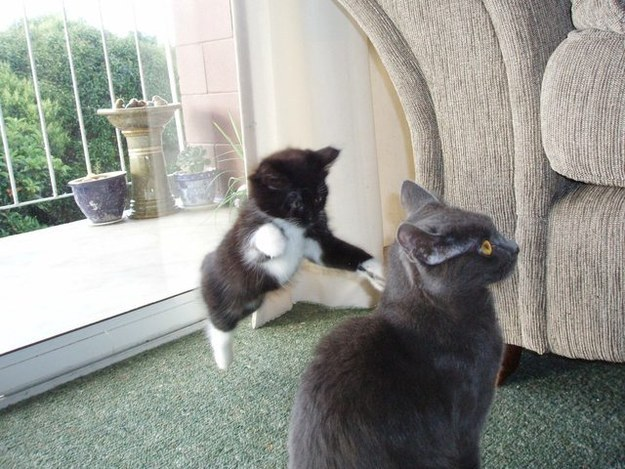
\includegraphics[scale=0.2]{img/0001.jpg}

\vsvitem{1-5:50}{}{appear}

\includegraphics[scale=0.2]{img/0002.jpg}

\vsvitem{1-06:00}{}{appear}
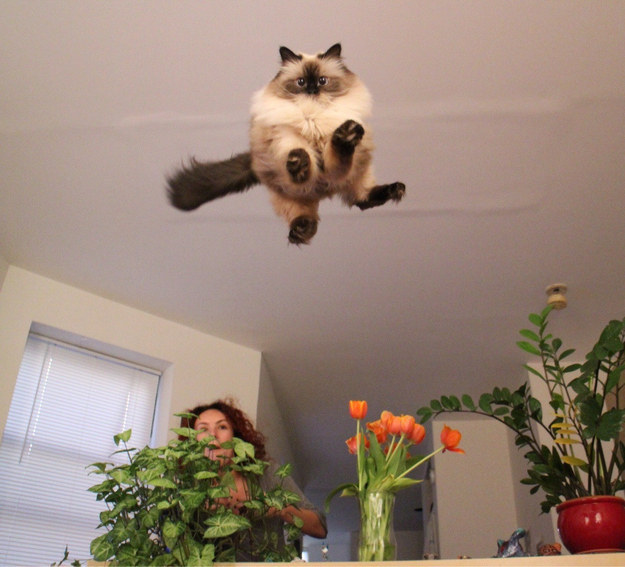
\includegraphics[scale=0.2]{img/0003.jpg}

\vsvitem{1-6:000000000000000010}{}{appear}
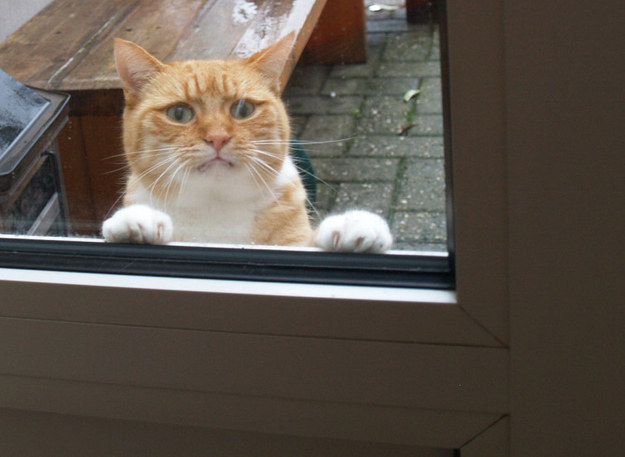
\includegraphics[scale=0.2]{img/0004.jpg}
\end{enumerate}

\begin{vsvappear}{1-00000000000000006:20}{}
And one final piece of text to appear!

\includegraphics[scale=0.2]{TODO}
\end{vsvappear}

\end{frame}

\begin{frame}{1-10:00.01}{2-5:00}{left}
\vsvhl{}{}{This is a cross-segment frame.}




% TODO do a strikethrough in a bullet point


\end{frame}

\input{vsv_template_footer.tex}

\end{document}
